\chapter{Inheriting XML Project Configuration Information}
\label{chapter:xml-inheritance}

As previously discussed, Opus uses XML-based configuration files to
flexibly specify the various aspects of a project, as well as to specify the
appearance of the different tabs in the GUI\@.

One configuration (the \emph{child}) can inherit from another configuration
(the \emph{parent}).  By default, the child inherits all the information
contained in the project.  However, it can override any information
inherited from the parent, and add additional information.  This means that
you can use default projects as parents for another project you want to
create that is mostly the same as an existing project, but has some changes
from it.  An XML configuration specifies its parent using the \emph{parent}
entry under the ``General'' section of the XML\@.  The value of this is the
name of the XML file that contains the parent configuration.  When
searching for this file, Opus first looks in the same directory that holds
the child configuration.  If it's not found there, it expects to find a
path in the Opus source code tree, starting with the name of a project like
\package{eugene} or \package{urbansim}.

This works well with the convention that users should create their own
projects in the \file{opus/project_configs} directory.  You can have
several configurations in your \file{opus/project_configs} directory, one
inheriting from the other.  Ultimately, though, one or more of these
configurations should inherit from a default configuration in the source
code tree in \file{opus/src}.  For example, Figure
\ref{fig:eugene-gridcell-xml-default} shows the contents of the
\file{eugene_gridcell_default.xml} project in \file{opus/project_configs}.  This
has almost no content of its own, but rather inherits everything but the
description from the parent configuration in the source code tree at
\file{eugene/configs/eugene_gridcell.xml}.

\begin{figure}[htp]
\begin{center}
\begin{verbatim}
<opus_project>
  <xml_version>4.2.0-beta1</xml_version>
  <general>
    <description type="string">Minimal user configuration for the Eugene gridcell project</description>
    <parent type="file">eugene/configs/eugene_gridcell.xml</parent>
  </general>
</opus_project>
\end{verbatim}
\end{center}
\caption{Contents of the default eugene\_gridcell.xml project}
\label{fig:eugene-gridcell-xml-default}
\end{figure}

A small section of its parent, \file{eugene/configs/eugene_gridcell.xml},
is shown in Figure \ref{fig:opus-xml}.  This is just a text file, but in a
structured format, with nodes corresponding to information that is
displayed in the GUI.  Some of the content of the XML provide data used by
the GUI to determine how to display information, or what menu items are
appropriate to connect to the node in the GUI.  Notice that this project in
turn inherits from \file{urbansim_gridcell/configs/urbansim_gridcell.xml}.

\begin{figure}[htp]
\begin{center}
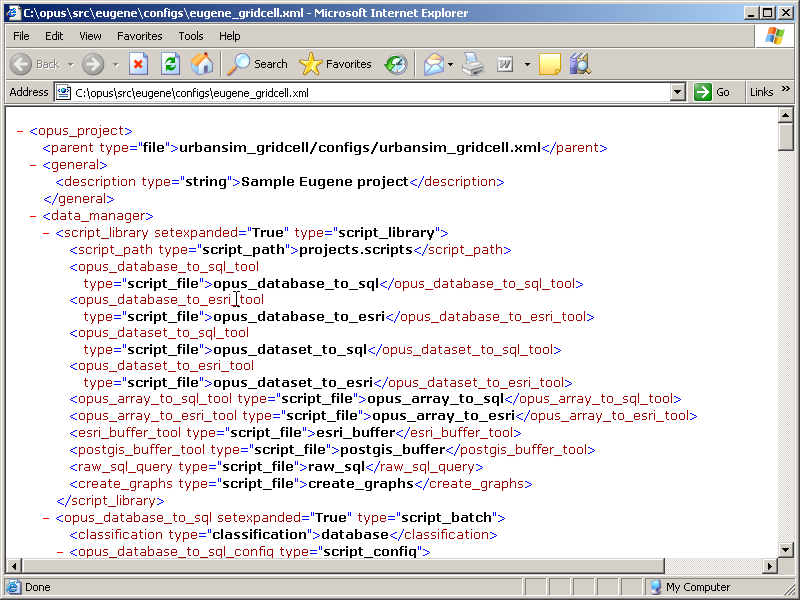
\includegraphics[scale=0.4]{graphics/opus-xml.png}
\end{center}
\caption{An Excerpt from eugene/configs/eugene\_gridcell.xml}
\label{fig:opus-xml}
\end{figure}

To change any of the options in the XML tree you need to be able to edit
it.  Inherited parts of the XML tree are shown in blue in the left pane in
the GUI\@.  These can't be edited directly --- they just show inherited
information.  You can make an inherited portion of the XML tree editable by
right clicking on it and selecting ``Add to curent project.''  This copies
the inherited information into the local XML tree, which then is shown in
black.  We saw an example of doing this in Section
\ref{sec:configuring-scenario}.  Figure
\ref{fig:scenario-manager-change-lastyear} in that same section shows an
XML tree that is mostly inherited (and so shown in blue).

A few details about the ``Add to current project'' command: in Section
\ref{sec:configuring-scenario}, when we added \code{lastyear} to the
current project, the containing nodes in the tree (\code{years_to_run} and
\code{Eugene_baseline}) also turned black, since they needed to be added to
the current project as well to hold \code{lastyear}.  It's also possible to
click directly on \code{years_to_run}, or even \code{Eugene_baseline}, and
add the XML tree under that to the current project.  However, we recommend
adding just the part you're editing to the current project, and not others.
(You can always add other parts later.)  The reason is that once a part of
the tree is added to the current project, the inheritance relation of that
part with the parent disappears, and changes to the parent won't be
reflected in the child XML\@.  For example, if you add all of the
\code{Eugene_baseline} node to the current project, save your
configuration, and then update the source code, changes to some obscure
advanced feature in the XML in the parent in the source tree wouldn't show
up in your configuration.

When you first start up the GUI and open a project, we suggested starting
with the default \file{eugene_gridcell_default.xml} configuration.  You can use the
``Save as'' command to save it under a new file name, and in that way keep
multiple configurations in your \file{opus/project_configs} directory.  You
can change the parent of a configuration by editing its parent field under
the ``General'' tab --- if you do this, save the configuration and then
re-open it so that the GUI will read in the new parent information (it
currently doesn't do that automatically).  Finally, since configurations
are just files, you can copy them, save them on a backup directory, or
email them as attachments to other users.  (You can also edit them directly
with a text editor --- but only do this if you know what you're doing,
since there won't be any checks that after your edits the configuration is
still well-formed.)

